% THE 1D QUANTUM WELL - THE PAULI EXCLUSION PRINCIPLE

\documentclass{standalone}



\IfStandalone{\def\datapath{../../../}}{\def\datapath{}}


\IfStandalone{\def\datapath{../../../}}{\def\datapath{}}

\usepackage{xcolor}
\definecolor{SciencePurple}{HTML}{663399}
\definecolor{ScienceBlue}{HTML}{214CCE}
\definecolor{ScienceGreen}{HTML}{007510}
\definecolor{ScienceYellow}{HTML}{ffbf00}
\definecolor{ScienceOrange}{HTML}{ff8c00}
\definecolor{ScienceRed}{HTML}{dc143c}
\usepackage{fontspec}
	\setmainfont{Roboto Slab}
	\setsansfont{Lato}
	\renewcommand{\familydefault}{\sfdefault}
	\setlength{\intextsep}{4pt} % Set defualt spacing around floats
	\definecolor{CommentGreen}{HTML}{228B22}
%	\captionsetup{aboveskip=5pt, belowskip=5pt} % Reduce space around captions

%% Math Env Text Settings
\usepackage{mathtools}
\usepackage{unicode-math}
	\setmathfont{XITS Math}
\usepackage{amsmath}
\usepackage{bm}
%	\everymath=\expandafter{\the\everymath\displaystyle}


%% https://tex.stackexchange.com/questions/8434/how-to-scale-math-font-only#8448
\DeclareMathSizes{11pt}{12pt}{7pt}{7pt}
\DeclareMathSizes{14pt}{15pt}{9pt}{9pt}

%% https://tex.stackexchange.com/questions/122574/globally-changing-math-line-spacing
\setlength{\jot}{7pt}

%% https://www.overleaf.com/learn/latex/Spacing_in_math_mode
%% https://tex.stackexchange.com/questions/41913/how-to-get-less-spacing-in-math-mode
%% https://mirror.kumi.systems/ctan/obsolete/info/math/voss/mathmode/Mathmode.pdf
\thinmuskip=5mu % (by default it is equal to 3 mu)
\medmuskip=5mu  % (by default it is equal to 4 mu)
\thickmuskip=7mu  % (by default it is equal to 5 mu)


\usepackage{tikz}
\usepackage{siunitx}
\usepackage{pgfplots}

\usepackage{physics}
\usepackage{etoolbox} %ifthen
\usepackage[outline]{contour} % glow around text


%%%%%%%%%% PGFPLOTS & PGFPLOTS SETTINGS %%%%%%%%%%
\pgfplotsset{compat=newest,
	width=6cm,
	height=3cm,
	scale only axis=true,
	max space between ticks=25pt,
	try min ticks=5,
	every axis/.style={
		axis y line=left,
		axis x line=bottom,
		axis line style={thick,->,>=latex, shorten >=-.4cm}
	},
	every axis plot/.append style={thick},
	tick style={black, thick}
}
\tikzset{
	semithick/.style={line width=0.8pt},
}

\usepgfplotslibrary{groupplots}
\usepgfplotslibrary{dateplot}

% https://tex.stackexchange.com/questions/441917/is-there-a-simple-way-to-use-stick-figures-into-pgf-tikz-drawings
\usepackage{tikzsymbols}
\usetikzlibrary{shapes.symbols}

\usetikzlibrary{calc}
\usetikzlibrary{arrows,arrows.meta,math}
\usetikzlibrary{decorations.markings}
\usetikzlibrary{angles,quotes} % for pic (angle labels)
\usetikzlibrary{fadings}

% https://tikz.dev/library-3d
\usetikzlibrary{3d}

% https://latexdraw.com/draw-a-sphere-in-latex-using-tikz/
\usepackage{tikz-3dplot}

% Define Color
\tikzstyle{bigphoton}=[-{Latex[length=8,width=6]},red!95!black!50,opacity=0.85,very thin,decorate,decoration={snake,amplitude=2.8,segment length=8,post length=8}]

\contourlength{1.4pt}




\begin{document}
	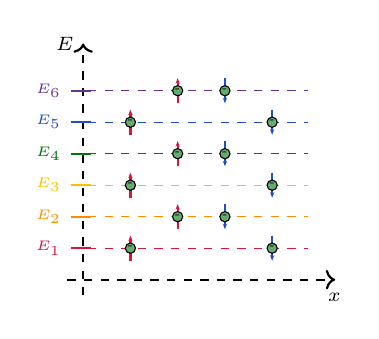
\begin{tikzpicture}
		\def\xmin{0} % min x axis
		\def\xmax{3}     % max x axis
		\def\BaseE{0.4}
		\def\L{2.85}
		\def\nSamples{100}
		
		
		\draw[->,thick,dashed] ({\xmin-0.2},0) -- ({\xmax+0.2},0) node[below=1] {\scriptsize $x$};
		\draw[->,thick,dashed] (\xmin,-0.2) -- (\xmin,{\BaseE*7.5}) node[above,left] {\scriptsize $E$} {};
		
		
		\draw[ScienceRed,thick] ({\xmin-0.15},\BaseE) node[left] {\tiny $E_1$} -- ({\xmin+0.1},\BaseE) {};
		\draw[ScienceOrange,thick] ({\xmin-0.15},{\BaseE*2}) node[left] {\tiny $E_2$} -- ({\xmin+0.1},{\BaseE*2}) {};
		\draw[ScienceYellow,thick] ({\xmin-0.15},{\BaseE*3}) node[left] {\tiny $E_3$} -- ({\xmin+0.1},{\BaseE*3}) {};
		\draw[ScienceGreen,thick] ({\xmin-0.15},{\BaseE*4}) node[left] {\tiny $E_4$} -- ({\xmin+0.1},{\BaseE*4}) {};
		\draw[ScienceBlue,thick] ({\xmin-0.15},{\BaseE*5}) node[left] {\tiny $E_5$} -- ({\xmin+0.1},{\BaseE*5}) {};
		\draw[SciencePurple,thick] ({\xmin-0.15},{\BaseE*6}) node[left] {\tiny $E_6$} -- ({\xmin+0.1},{\BaseE*6}) {};
		
		\draw[ScienceRed,dashed] ({\xmin-0.15},\BaseE) -- (\L,\BaseE) {};
		\draw[ScienceOrange,dashed] ({\xmin-0.15},{\BaseE*2}) -- (\L,{\BaseE*2}) {};
		\draw[ScienceYellow,dashed] ({\xmin-0.15},{\BaseE*3}) -- (\L,{\BaseE*3}) {};
		\draw[ScienceGreen,dashed] ({\xmin-0.15},{\BaseE*4}) -- (\L,{\BaseE*4}) {};
		\draw[ScienceBlue,dashed] ({\xmin-0.15},{\BaseE*5}) -- (\L,{\BaseE*5}) {};
		\draw[SciencePurple,dashed] ({\xmin-0.15},{\BaseE*6}) -- (\L,{\BaseE*6}) {};
		
		\begin{scope}
			\foreach \i in {1,...,6}{
				\ifodd\i
					\draw[-{Stealth[length=2pt]},thick,ScienceRed] ({\xmax*0.2},{(\i*\BaseE)-(\BaseE*0.4)}) -- ({\xmax*0.2},{(\i*\BaseE)+(\BaseE*0.4)});
					\draw[-{Stealth[length=2pt]},thick,ScienceBlue] ({\xmax*0.8},{(\i*\BaseE)+(\BaseE*0.4)}) -- ({\xmax*0.8},{(\i*\BaseE)-(\BaseE*0.4)});
					
					\draw[fill=ScienceGreen!60] ({\xmax*0.2},{\i*\BaseE}) circle [radius = 0.065];
					\node[anchor=center] at ({\xmax*0.2},{\i*\BaseE}) {\tiny -};
					
					\draw[fill=ScienceGreen!60] ({\xmax*0.8},{\i*\BaseE}) circle [radius = 0.065];
					\node[anchor=center] at ({\xmax*0.8},{\i*\BaseE}) {\tiny -};
					
				\else
					\draw[-{Stealth[length=2pt]},thick,ScienceRed] ({\xmax*0.4},{(\i*\BaseE)-(\BaseE*0.4)}) -- ({\xmax*0.4},{(\i*\BaseE)+(\BaseE*0.4)});
					\draw[-{Stealth[length=2pt]},thick,ScienceBlue] ({\xmax*0.6},{(\i*\BaseE)+(\BaseE*0.4)}) -- ({\xmax*0.6},{(\i*\BaseE)-(\BaseE*0.4)});
					
					\draw[fill=ScienceGreen!60] ({\xmax*0.4},{\i*\BaseE}) circle [radius = 0.065];
					\node[anchor=center] at ({\xmax*0.4},{\i*\BaseE}) {\tiny -};
					
					\draw[fill=ScienceGreen!60] ({\xmax*0.6},{\i*\BaseE}) circle [radius = 0.065];
					\node[anchor=center] at ({\xmax*0.6},{\i*\BaseE}) {\tiny -};
				\fi
			}
		\end{scope}
		
	\end{tikzpicture}
\end{document}